\section{Implementations}  
\label{implementations}

Almost every researcher studying the theory or one of the applications of the Tutte polynomial (or any of its specialisations) will --- at least occasionally --- wish to explicitly compute the Tutte polynomial of a specific graph or matroid. In this chapter we survey the options easily
available to a researcher in this position, although these options are very limited indeed for the matroid-theorist.

There is a vast statistical physics literature devoted to the computation of the partition function of the $q$-state Potts model for particular
families of graphs, usually (but not always) strips or portions of regular lattices of various types. Many of these papers describe ingenious implementations based on transfer matrix methods, compute the partition functions, and then analyse the resulting polynomials and their complex roots to shed light on physical or mathematical questions. 

While these methods will significantly outperform {\em any} general-purpose computational tool, they apply only to the small classes of graphs
for which they were explicitly designed, and hence in this chapter we largely omit any reference to this literature despite its importance; our focus
will purely be on the computational tools applicable to any graph (or matroid) with no {\em a priori} structural constraints.

The matroid theorist has only one widely-available tool --- the method \verb+tutte_polynomial()+ in the package \verb+sage_matroids+
which is distributed with the open-source Sage computer algebra system (available at \url{http://sagemath.org/}).  This is a naive algorithm that, while optimised, involves enumerating each base of the matroid and determining its internal and external activity. Therefore the time taken primarily depends on the number of bases of the matroid.

%\[
%T_G(x,y) = (x-1)^{-c} (y-1)^{-|V|} Z_G((x-1)(y-1),y-1)
%\]
%
%\[
%Z_G(q,v) = q^c v^{|V|-c} \ T_G \left( \frac{q}{v}+1,v+1 \right)
%\]
%
%\[
%Z_G^\text {Potts}(q,\mathbf{v}) = \sum_{\sigma: V \rightarrow \{1,2,\ldots,q\}} \prod_{e=xy} \left( 1 + v_e \delta(\sigma(x),\sigma(y)) \right)
%\]

\subsection{Haggard, Pearce \& Royle (HPR)}

Haggard, Pearce \& Royle have implemented a program to calculate the Tutte polynomial based on the standard  deletion-contraction recurrence
\[
T_G(x,y) = 
\begin{cases}
1 & \text{if $G$ has no edges},\\
T_{G \backslash e}(x,y) + T_{G/e} (x,y) & e \text{ not a loop or coloop},\\
x T(G/e, x, y) & e \text{ is a coloop,}\\
y T(G\backslash e, x, y) & e \text{ is a loop,}\\
\end{cases}
\]
where $G/e$ and $G\backslash e$ are the graphs arising by {\em contracting} $e$ or {\em deleting} $e$ respectively, retaining any loops or multiple edges that may be created. 

The program then performs a depth-first search on the search tree implied by the deletion-contraction algorithm. During this process some graphs may be encountered that are isomorphic to graphs that have previously been processed to completion, and so a naive implementation of deletion-contraction
potentially repeats computations unnecessarily. To avoid this, the HPR algorithm maintains a {\em cache} storing the canonically-labelled isomorphs of the 	`most recently-encountered intermediate graphs along with their Tutte polynomials. At every node of the search tree, the graph currently being processed is canonically labelled (using Brendan McKay's program \verb+nauty+  \cite{MR3131381}) and compared to those in the cache. If the graph is already in the cache, then the stored Tutte polynomial is re-used, rather than being re-computed.

The cache dramatically improves the performance, but in a rather unpredictable manner. The success of this strategy is determined by the number of beneficial collisions in the cache, which depends on a variety of user-selectable parameters such as the cache size, the cache-removal mechanism, the edge-selection heuristic and the initial labelling of the graph. 

\subsection{Bedini \& Jacobsen (BJ)}

Bedini and Jacobsen \cite{BJ10} have implemented a program to calculate the partition function $Z_G(q,v)$ of the $q$-state Potts model which, in the Fortuin-Kastelyn expansion, can be defined as follows:
\begin{equation}\label{zqv}
Z_{G}(q,v) = \sum_{A \subseteq E(G)} v^{|A|} q^{c(A)}
\end{equation}
where $c(A)$ denotes the number of connected components of the graph $(V(G),A)$, i.e., the graph with all the vertices of $G$, but only the edges in $A$. Although the partition function $Z_G$ is equivalent to the Tutte polynomial, this formulation is preferred by mathematical physicists because of the fundamentally different roles played by $q$ and $v$ in the Potts model. Fortunately converting between the Tutte polynomial and the partition function of the $q$-state Potts model requires only simple variable substitution:
\begin{align*}
Z_G(q,v) &= q^{c(G)} v^{|V|-c(G)} \ T_G \left( q/v +1,v+1 \right),\\
T_G(x,y) &= (x-1)^{-c(G)} (y-1)^{-|V|} Z_G((x-1)(y-1),y-1).
\end{align*}

Statistical physicists are often concerned with the behaviour of the partition function on various structured families of graphs 
$\mathcal{G} = \{G_n\}$ such that $|V(G_n)| \rightarrow \infty$ as $n \rightarrow \infty$. In particular, the families most often 
studied by physicists are various types of {\em lattice} where one dimension is fixed while the other dimension
increases. %The boundary conditions, either ``periodic'' or ``free'', specify that the edges of the lattice wrap around or do not wrap around, respectively.

\begin{figure}
\begin{center}
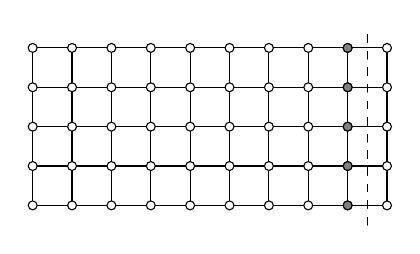
\begin{tikzpicture}[scale=0.5]
\tikzstyle{vertex}=[circle, draw=black, fill=white, inner sep = 0.4mm]
\tikzstyle{gvertex}=[circle, draw=black, fill=gray, inner sep = 0.4mm]
%\draw (0,0) grid (8,4);
%\foreach \x in {0,1,...,8} 
%\foreach \y in {0,1,...,4} {
%\node [vertex] at (\x,\y) {};
%}
%
%\pgftransformxshift{11cm}

\draw (0,0) grid (9,4);
\foreach \x in {0,1,...,9} 
\foreach \y in {0,1,...,4} {
\node [vertex] at (\x,\y) {};
\draw [dashed] (8.5,-0.5)--(8.5,4.5);
}

\foreach \y in {0,1,...,4} {
\node [gvertex] at (8,\y) {};
}


\end{tikzpicture}
\end{center}
\caption{Adding a layer to  a section of the square lattice}
\label{extending}
\end{figure}

%\begin{figure}
%\begin{center}
%\begin{tikzpicture}[scale=0.5]
%\tikzstyle{vertex}=[circle, draw=black, fill=white, inner sep = 0.4mm]
%\draw (0,0) grid (8,4);
%\foreach \x in {0,1,...,8} 
%\foreach \y in {0,1,...,4} {
%\node [vertex] at (\x,\y) {};
%}
%\pgftransformxshift{11cm}
%
%\draw (0,0)--(8,0);
%\draw (0,2)--(8,2);
%\draw (0,4)--(8,4);
%\draw (0.5,1)--(8.5,1);
%\draw (0.5,3)--(8.5,3);
%
%\draw (0,0)--(2,4);
%\draw (1,0)--(3,4);
%\draw (2,0)--(4,4);
%\draw (3,0)--(5,4);
%\draw (4,0)--(6,4);
%\draw (5,0)--(7,4);
%\draw (6,0)--(8,4);
%
%\draw (8,0)--(6,4);
%\draw (7,0)--(5,4);
%\draw (6,0)--(4,4);
%\draw (5,0)--(3,4);
%\draw (4,0)--(2,4);
%\draw (3,0)--(1,4);
%\draw (2,0)--(0,4);
%\draw (0,2)--(1,4);
%\draw (0,2)--(1,0);
%\draw (8,2)--(7,4);
%\draw (8,2)--(7,0);
%\draw (8,0)--(8.5,1)--(8,2)--(8.5,3)--(8,4);
%
%\foreach \x in {0,1,...,8}
%\foreach \y in {0,2,4} 
%\node [vertex] at (\x,\y) {};
%
%\foreach \x in {0.5,1.5,...,8.5}
%\foreach \y in {1,3} 
%\node [vertex] at (\x,\y) {};
%
%\end{tikzpicture}
%\end{center}
%\caption{Sections of the square lattice and triangular lattice.}
%\end{figure}

In these cases, the lattice is viewed as being built up layer-by-layer, with each new layer attaching to the {\em boundary vertices} of the previous graph.  By keeping some auxiliary information, it is possible to incrementally update the partition function as each new layer is added. The auxiliary information kept are the {\em partial partition functions} defined as follows: Each subset $A$ of edges in the expression \eqref{zqv} determines a {\em partition} of the boundary vertices where two vertices are in the same cell if they are connected by edges in $A$. The partial partition function $Z_G^\pi$ associated to $\pi$ is the total contribution to $Z_G$ made by all edge subsets with boundary partition $\pi$. Thus we have the sum
\[
Z_G (q,v) = \sum_\pi Z_G^\pi (q,v),
\]
where $\pi$ ranges over all the partitions of the boundary vertices.

Now suppose that a new layer is added to the graph $G$ forming a larger graph $G'$, and consider $Z_G'(q,v)$. We aim to show that all the partial partition functions $Z_{G'}^{\pi'}$ can be calculated from the partial partition functions of $G$.  So consider an arbitrary  subset of $E(G')$, expressing it as $A \cup A'$, where $A \subseteq E(G)$ and $A'$ is a subset of the newly added edges. The graph $(V(G),A)$ has a particular number of edges and connected components, and determines a particular partition $\pi$ of the old boundary vertices. After adding the edges $A'$, the number of edges and connected components of $(V(G'),A \cup A')$ changes, and a partition $\pi'$ of the new boundary vertices is created. The key point is that these changes are determined {\em only} by the partition $\pi$ and the subset $A'$, and not by the exact subset $A$. Therefore for each boundary partition $\pi'$ of $G'$, the partial partition function $Z_{G'}^{\pi'}$ is a linear combination (whose coefficients are polynomials in $q$, $v$) of the partial partition functions $Z_G^\pi$.  
The {\em transfer matrix} $T$ is a matrix whose rows and columns are indexed by partitions of the old boundary vertices and new boundary vertices respectively, and whose entries contain these polynomials. If $v$ is a (column) vector indexed by partitions of the boundary vertices, such that $v_\pi$ is the partial partition function associated with $\pi$, then $Tv$ is the same vector for the graph with one layer added. If each layer has the same structure, as is the case for regular lattices, then this process can be {\em iterated}, in which case $T^mv$ is the result of adding $m$ layers. In this simple situation, the long term behaviour is determined by spectral properties of $T$.

Bedini \& Jacobsen's algorithm is based on applying the underlying principles of the transfer matrix method to graphs with no {\em a priori} layered structure. In its simplest form, their algorithm processes a graph vertex-by-vertex, maintaining a ``boundary'' between the processed and unprocessed vertices, along with the partial partition functions indexed by the boundary partitions. The boundary evolves as the algorithm runs, and it will grow and shrink as each vertex is included, processed, and then removed.  As every boundary partition must be analysed and processed, it is important to keep the boundary as small as possible throughout the process. In order to achieve this, they have implemented a much more sophisticated variant of this basic idea based on the concept of a {\em tree decomposition}. A tree decomposition of a graph $G$ is a tree $T$ whose vertices are labelled by subsets of $V(G)$ called {\em bags}, such that the two vertices of each edge are contained in at least one bag, and for each vertex $v$ of $G$, the subgraph of $T$ induced by the bags containing $v$ is a connected subtree of $T$. The {\em tree-width} of a graph is one less than the minimum over all tree decompositions of the maximum bag size in that decomposition. As its name suggests, the tree-width can be viewed as measuring how ``tree-like'' a graph is. In particular, the graphs of tree-width one are exactly trees, while graphs of tree-width two are series-parallel graphs. 

The algorithm starts by heuristically finding a ``good'' tree decomposition for the graph (finding an optimal tree decomposition is NP-hard), and then using that tree decomposition to determine the order in which the vertices are processed, with the maximum bag size determining the maximum boundary size that will be encountered during this process. (Details of how the algorithm deals with gluing together the recursively calculated partial partition functions at a tree vertex of degree more than two are omitted here, but may be found in \cite{BJ10}.)

Thus, if a graph is qualitatively tree-like --- that is, somewhat ``long and skinny'' --- then the approximation algorithm will find a tree decomposition with small maximum bag size and the algorithm will run very fast, even for large graphs. However if the graph has large tree-width, then {\em every} tree decomposition will have some large bags and both the time and space requirements will increase accordingly. More importantly however, the user need not know whether their graph is tree-like or not --- if the algorithm is presented with an ``easy'' graph, then this will be detected without explicit user intervention, and the running time will reflect this.

Overall, this algorithm appears to be extremely effective, particularly for relatively sparse graphs (such as planar graphs). 

\subsection{Bj\"orklund, Husfeldt, Kaski \& Koivisto (BHKK)}

Bj\"orklund, Husfeldt, Kaski \& Koivisto take a completely different approach to the computation of the Tutte polynomial. Their paper is largely concerned with proving that the Tutte polynomial $T_G$ can be calculated in time exponential in the number of vertices of $G$, which was not previously known. They describe two algorithms to achieve this, and provide an implementation of one of them, which is ultimately based on manipulating subsets of the {\em vertices} of the graph, rather than subsets of edges.

The starting point is to consider a different expression for the partition function of the $q$-state Potts model, where $q$ is taken to 
a fixed, but otherwise arbitrary, positive integer. So we define
\begin{equation}\label{zqvpotts}
Z_G^{\mathrm{Potts}} (q,v) = \sum_{\sigma:V \rightarrow \{1,2,\ldots,q\}} \prod_{e = xy} \left( 1+v \delta(\sigma(x),\sigma(y) \right),
\end{equation}
where the sum is taken over all $q$-colourings $\sigma$ (proper or improper), the product is taken over all edges $e \in E(G)$ and $\delta$ is the Kronecker delta. In other words, a $q$-colouring with $m$ monochromatic edges contributes $(1+v)^m$ to the sum. This formulation reflects the physical basis of the partition function of the $q$-state Potts model as a sum over all possible states of a graph when each vertex takes one of $q$ possible ``spins''. Fortuin \& Kastelyn \cite{MR0359655} first proved the equivalence of \eqref{zqv} and \eqref{zqvpotts}.

Each colouring $\sigma$ determines a partition of $V(G)$ into colour classes, and each term of the sum depends on the number of edges contained in the induced subgraphs on each colour class. For $X \subseteq V(G)$, let $G[X]$ denote the subgraph of $G$ induced by the vertices in $X$, let $m(X)$ denotes the number of edges of $G[X]$, and let $f(X) = (1+v)^{m(X)}$.
Then
\begin{equation}\label{zqvpart}
Z_G (q,v) = \sum_{(X_1, X_2, \ldots, X_q)} \prod_{i=1}^q f(X_i),
\end{equation}
where the summation is over all {\em ordered partitions} $(X_1, X_2, \ldots, X_q)$ of $V$, where an ordered partition is a sequence of
pairwise-disjoint subsets whose union is $V$.

The BHKK algorithm proceeds by {\em numerically evaluating} this expression for $1 \leq v \leq m-n+2$ and $2 \leq q \leq n$ (where  
$G$ has $n$ vertices and $m$ edges) and then using Lagrange interpolation to determine the coefficients of the
Tutte polynomial. To avoid manipulation of arbitrary length integers as much as possible, the calculations are done in $\mathbb{Z}_p$ where
$p$ is a large prime, and then repeated for as many additional primes as necessary to use the Chinese Remainder Theorem to 
unambiguously determine the coefficients.

We need some more terminology before explaining exactly {\em how} \eqref{zqvpart} is evaluated. So suppose that $f:2^V \rightarrow R$ is
a function from subsets of $V$ to a ring $R$ (think of $R$ as some $\mathbb{Z}_p$).  Then the {\em $\zeta$-transform} of $f$, denoted $f\zeta$, is the function $f\zeta: 2^V \rightarrow R$ given by
\[
(f\zeta) (X) = \sum_{X' \subseteq X} f(X'),
\]
or in other words, the sum of $f$ over all subsets of $X$ (including $\emptyset$ and $X$ itself).  The {\em M\"obius transform} of $f$, denoted $(f\mu)$, is the function 
$f\mu: 2^V \rightarrow R$ such that 
\[
(f\mu)(X) = \sum_{X' \subseteq X} (-1)^{|X\backslash  X'|} f(X'),
\]
and it is the inverse of the $\zeta$-transform. The rationale for introducing these functions is that it is known that
\begin{equation}\label{zqvcover}
\left( (f\zeta)^q \mu \right) (V) = \sum_{(X_1, X_2, \ldots, X_q)} \prod_{i=1}^q f(X_i),
\end{equation}
where the summation is over all {\em ordered covers} $(X_1, X_2, \ldots, X_q)$ of $V$ and  $(f\zeta)^q$ means the point wise $q$-th power of $(f\zeta)$. Importantly, note that an ordered cover is a sequence of subsets --- {\em not necessarily pairwise-disjoint} --- whose union is $V$.

Comparing \eqref{zqvcover} and \eqref{zqvpart} we see \eqref{zqvcover} includes all the terms of \eqref{zqvpart}, along with many extra terms. However BHKK found a clever way to extract precisely the required information from \eqref{zqvcover}. They introduced a new indeterminate $z$ and a new function $f_z: 2^V \rightarrow R[z]$ defined by 
\[
f_z(X) = (1+v)^{m(X)} z^{|n(X)|}
\]
which is a monomial (in $z$) in the polynomial ring $R[z]$. In other words, the value  $f_z(X)$ now carries information about the {\em size} of $X$ in addition to the value $f(X)$. Therefore the expression $\left( (f\zeta)^q \mu \right) (V)$ is a polynomial in $z$. An ordered cover $(X_1, X_2, \ldots, X_q)$ contributes to the coefficient of $z^n$ if and only if $n(X_1) + n(X_2) + \cdots + n(X_q) = n$, in which case the {\em cover} is necessarily a {\em partition}. Therefore the value we are seeking is {\em precisely} the coefficient of $z^n$ in $((f_z \zeta)^k \mu) (V)$.

Thus a simplified overview of the overall strategy of the BHKK algorithm is that it first fixes a specific value for $v$, then computes the (polynomial-valued) function $(f_z \zeta)$ (that is, it is calculated for each subset of $V(G)$). Then by polynomial multiplication, each of $(f_z \zeta)^2$, $(f_z \zeta)^3$, $\ldots$, $(f_z \zeta)^n$ is calculated. During this procedure, the contribution that each subset will ultimately make to the $z^n$ coefficient of $((f_z \zeta)^k \mu) (V)$ is calculated
and accumulated. There are some obvious optimisations that can be made --- for example, every polynomial can be truncated after the $z^n$ term, because no higher order terms can arise from ordered partitions. In the actual implementation, some additional clever optimisations speed up various aspects of the overall strategy, but we omit the details here.

The BHKK algorithm is competitive for relatively small, but dense, graphs, but as the number of vertices increases, it becomes unusably slow. The reason for this is clear from the nature of the algorithm --- each of the functions $f_z$ and its various transforms and powers is stored in image form, i.e, as an array of $2^n$ polynomials in $z$, and each evaluation involves processing the entire array.

%The starting point is to rewrite Equation~\eqref{zqv} so that the summation is taken over all the subsets $A \subseteq E(G)$ such that $(V(G),A)$ has $k$ connected components, where $1 \leq k \leq n$ 
%
%\begin{equation}\label{newone}
%Z_G(q,v) = \sum_{k=1}^{k=n} q^k S_G(k, v)
%\end{equation}
%where for $1 \leq k \leq n$, 
%\begin{equation}
%S_G(k, v) = \sum_{\substack{A \subseteq E \\ c(A) = k}} v^{|A|}.
%\end{equation}
%
%For $k \geq 2$, the values $S_G(k,v)$ can calculated recursively by observing that any subgraph with $k$ components can be split into a connected subgraph and one with $k-1$ components. In particular, if $G[W]$ denotes the graph induced
%by a vertex-subset $W \subseteq V(G)$, then 
%\begin{equation}
%S_{G[W]} (k,v) = \frac{1}{k} \sum_{\emptyset \neq U \subset W} S_{G[U]} (1,v) S_{G[W\backslash U]} (k-1,v).
%\end{equation}
%
%This leaves only the case where $k=1$, corresponding to a connected subgraph, and for this we can subtract the disconnected subgraphs from the total number of subgraphs.
%\begin{equation}
%S_{G[W]} = (1+v)^{|E(G[W])|} - \sum_{k\geq 2} S_{G[W]} (k,v) 
%\end{equation}
%
%However they do not attempt to manipulate this symbolically (thus maintaining 
%
%An interesting feature of their method is that rather than manipulating polynomials symbolically (i.e., storing the coefficients), their program manipulates the {\em values} $Z_G(q,v)$ for all  $1 < q < n$ and $1 \leq v \leq e-n+2$ and then uses Lagrange interpolation to recover the coefficients of the Tutte polynomial from these values. In addition, rather than carrying these values as arbitrary-precision integers using GMP (which has considerable overhead) or similar, the calculations are instead done over the ring of integers $Z_p$, where $p$ is some large prime that fits into a single machine word. If necessary, the calculations are then repeated using a different prime $p'$ and so on, until the Chinese Remainder Theorem can be used to determine the coefficients exactly. 

